
\section{Zasoby i zarządzanie nimi}
\label{sec:zasoby}


Gospodarka składa się z zon, zasobów oraz grup politycznych. Naturalnie w przyrodzie występują tylko zasoby surowcowe (S). Przestrzeń gospodarki jest podzielona na zony (Z). Do zon przypisane są zasoby surowcowe. Oznaczenie zasobu obejmuje symbol zasobu oraz jego poziom. Poziom to ilość zasobu, który można wydobyć w jednej turze. [opt. zasoby surowcowe są wyczerpywalne, więc ich poziom maleje w czasie]. Z zasobów surowcowych można produkować zasoby wyższego poziomu, przemysłowe oraz high-tech (rys.\ref{fig:zasoby}). 
Zasoby mogą być wymieniane pomiędzy grupami politycznymi (handel) lub pomiędzy zonami (składowanie).

\begin{figure}[h!]
    \centering
    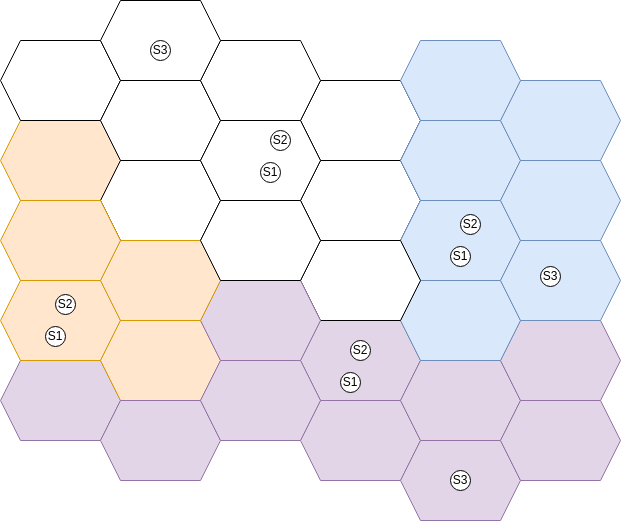
\includegraphics[width=0.8\textwidth]{img/zony.drawio.png}
    \caption{Przykład podziału przestrzeni na zony jako siatka hexagonalna, z przypisanymi zasobami}
    \label{fig:zony}
    \end{figure}


Grupa polityczna zajmuje określone zony, przez co i zasoby (rys. \ref{fig:zony}).Celem grupy politycznej jest zdobycie jak największej ilości zasobów, aby produkować zasoby wyższego poziomu i zdobywać przewagę nad innymi grupami politycznymi.


Grupa polityczna ma dwa rodzaje interakcji z innymi grupami politycznymi:
\begin{itemize}
    \item \textbf{Interakcje pokojowe} - grupy polityczne mogą tworzyć sojusze, wymieniać się zasobami, aby produkować zasoby wyższego poziomu (opcjonalne).
    \item \textbf{Interakcje militarne} - grupy polityczne mogą atakować inne grupy polityczne, aby zdobyć ich zony i zasoby.
\end{itemize}





\begin{figure}[h!]
\centering
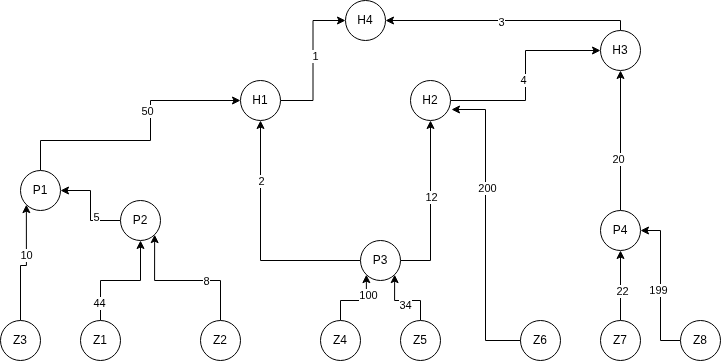
\includegraphics[width=0.8\textwidth]{img/zasoby.drawio.png}
\caption{Schemat zasobów. Liczby oznaczają ile jednostek zosobu jest potrzebne do produkcji 1 jednostki zasobu wyższego poziomu.}
\label{fig:zasoby}
\end{figure}




\subsection{Przykład 1 }

\subsubsection{Przygotowanie}

\begin{itemize}
    \item Przygotuj graf zasobów.
    \item Przygotuj graf gospodarek, państw.
    \item Przygotwuj cennik zasobów.
\end{itemize}

\subsubsection{Przebieg rozgrywki 1. - tylko militarna}




Rozgrywka składa się z tur, w których grupy polityczne wykonują swoje ruchy. 

Każda tura składa się z kilku faz:
\begin{itemize}
    \item Każda GP oblicza jakie zasoby ma i jakie zasoby może produkować.
    \item Każda GP sprawdza jakie zasoby mogłaby mieć gdyby pokonała inne GP i przejęła ich zony. Sprawdza to dla każdego sąsiada.
    \item Każda GP decyduje o kierunku ataku. Atakuje sąsiada, który ma najwięcej zasobów, które GP może zdobyć, a który jednocześnie jest najsłabszy. 
    \item  Kolejność ataków jest ustalana losowo. Jeśli jakiś GP chce zaatakować sąsiada, który już został zaatakowany i pokonany to dany atak jest pomijany.
    \item Potencjał przeciwników jest określany w momencie ataku. To znaczy, że jeśli jakiś GP w między czasie pokonał innego GP to może się okazać, że początkowo słabszy GP stał się silniejszy i nie można go pokonać.
\end{itemize}
Z poniższej tabelki wynika, że GP A atakuje GP c, ale GP b również atakuje GP c. Więc tu następuje losowanie.
W tej tabelce trzeba dodać potencjały ekonomiczne.

    \begin{table}[h!]
    \centering
    \begin{tabular}{|c|c|c|c|}
    \hline
    \textbf{atakujący A} & \textbf{atakowany D} & \textbf{potencjał militarny A}  & \textbf{potencjał mil. D}\\ \hline
    a & b & 10 & 20 \\ \hline
    a & c & 10 & 8 \\ \hline
    b & c & 20 & 8 \\ \hline
    c & a & 8 & 10 \\ \hline
    \end{tabular}
    \caption{Rodzaje zasobów w grze i ich przykłady}
    \label{tab:zasoby}
    \end{table}



\subsection*{Inne możliwości}

\begin{itemize}
    \item Niektóre zasoby na początku rozgrywki nie są przypisane do żadnej grupy politycznej. Grupa polityczna może je zdobyć, zajmując odpowiednią zonę.
    \item Zosoby są wyczerpywalne, są magazynowane, mają okres przydatności itp.
    \item Produkcja zasobów zajmuje czas, transport zasobów zajmuje czas, itp.
    \item Wprowadzenie modeli makroekonomicznych, które będą wpływały na zasoby i ich produkcję.


\end{itemize}